\documentclass{standalone}
\usepackage{tikz}
\usetikzlibrary{positioning,shapes,shadows,arrows}

\begin{document}
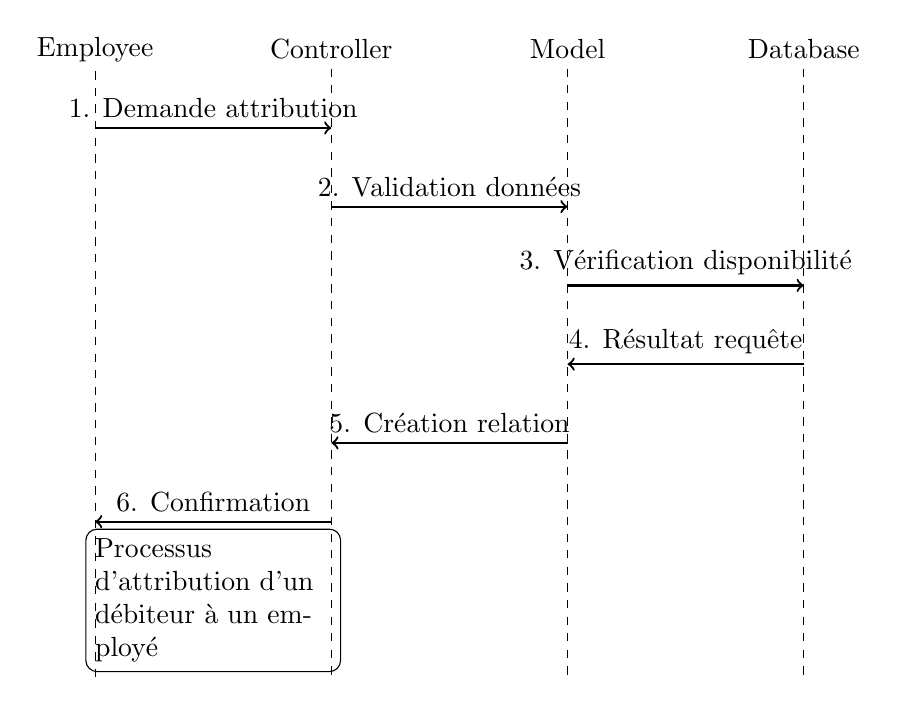
\begin{tikzpicture}[
    lifeline/.style={draw, dashed},
    message/.style={->, thick},
    note/.style={draw, rectangle, rounded corners, text width=3cm}
]

% Lifelines
\node (employee) at (0,0) {Employee};
\node (controller) at (3,0) {Controller};
\node (model) at (6,0) {Model};
\node (database) at (9,0) {Database};

% Lifeline vertical lines
\draw[lifeline] (employee) -- (0,-8);
\draw[lifeline] (controller) -- (3,-8);
\draw[lifeline] (model) -- (6,-8);
\draw[lifeline] (database) -- (9,-8);

% Messages
\draw[message] (0,-1) -- node[above] {1. Demande attribution} (3,-1);
\draw[message] (3,-2) -- node[above] {2. Validation données} (6,-2);
\draw[message] (6,-3) -- node[above] {3. Vérification disponibilité} (9,-3);
\draw[message] (9,-4) -- node[above] {4. Résultat requête} (6,-4);
\draw[message] (6,-5) -- node[above] {5. Création relation} (3,-5);
\draw[message] (3,-6) -- node[above] {6. Confirmation} (0,-6);

% Notes
\node[note] at (1.5,-7) {Processus d'attribution d'un débiteur à un employé};

\end{tikzpicture}
\end{document} 